\documentclass{article}
\usepackage[margin=1in]{geometry}
\usepackage{fancyhdr}
\pagestyle{fancy}
\lhead{}
\chead{}
\rhead{Mermin (2007) \textit{Quantum Computer Science}}
\lfoot{}
\cfoot{\thepage}
\rfoot{}
\usepackage{amsmath, amsthm, amssymb}
\usepackage{bm} % for bold math symbols
\usepackage{mathtools}
\usepackage{graphicx}
\usepackage{caption}
\usepackage{hyperref}
\usepackage{changepage}
\usepackage{lipsum}
\usepackage{color, colortbl} % For Coloring Table Elements
\usepackage{wrapfig}
%\usepackage{alltt}
\usepackage{listings}
\usepackage{makecell} % allows more complex table formatting
\usepackage{proof} %for inference trees
\usepackage{scrextend} % for block indents (for example)
%\usepackage{cite} % incompatible with biblatex
\usepackage{biblatex}
\addbibresource{bibliography.bib}
\def\BibTeX{{\rm B\kern-.05em{\sc i\kern-.025em b}\kern-.08em
    T\kern-.1667em\lower.7ex\hbox{E}\kern-.125emX}}
\usepackage{url}

% for the makecell package:
\renewcommand\theadalign{bc}
\renewcommand\theadfont{\bfseries}
\renewcommand\theadgape{\Gape[4pt]}
\renewcommand\cellgape{\Gape[4pt]}

\addtolength{\hoffset}{-1cm}
\addtolength{\textwidth}{1cm}
\graphicspath{ {IMAGES/} }

\definecolor{Gray}{gray}{0.9}
\newcolumntype{g}{>{\columncolor{Gray}}c}

\title{Notes \& Elaborations on Mermin's (2007) \textit{Quantum Computer Science: An Introduction}}
\author{Warren (Hoss) Craft}
\date{Summer 2019}

\begin{document}
\maketitle
%\tableofcontents
%\newpage

\flushleft

%%%%%%%%%%%%%%%%%%%
%   1.35          %
%%%%%%%%%%%%%%%%%%%

\textbf{EQ 1.35 (SWAP operator in terms of projections and flips)}\par

\vspace{0.125in}

On pg 12, Mermin \cite{Mermin:2007} notes that the SWAP operator $S_{ij}$ can be written as:
\[\tag{1.35}
    \bm{S}_{ij} = \bm{n}_i \bm{n}_j
    + \bm{\widetilde{n}}_i \bm{\widetilde{n}}_j
    + (\bm{X}_i \bm{X}_j)
      ( \bm{n}_i \bm{\widetilde{n}}_j 
        + \bm{\widetilde{n}}_i \bm{n}_j)
\]
and he goes on to remark that:
\vspace{0.125in}
\begin{addmargin}[0.25in]{0.25in}
At the risk of belaboring the obvious, I note that (1.35) acts as the swap operator because if both Cbits are in the state $|1\rangle$ (so swapping their states does nothing) then only the first term in the sum acts (\textit{i.e.} each of the other three terms gives 0) and multiplies the state by 1; if both Cbits are in the state $|0\rangle$, only the second term acts and again multiplies the state by 1; if Cbit $i$ is in the state $|1\rangle$ and Cbit $j$ is in the state $|0\rangle$, only the third term acts and the effect of flipping both Cbits is to swap their states; and if Cbit $i$ is in the state $|0\rangle$ and Cbit $j$ is in the state $|1\rangle$, only the fourth term acts and the effect of the two $X$s is again to swap their states.
\end{addmargin}

\vspace{0.125in}

Mermin's comment that ``each of the other three terms gives 0'', for example, can be confusing, and the interpretation of the summation operations could use some clarification as well. To see more clearly what is happening in (1.35), it can help to consider the SWAP operator $S_{01}$ (and its equivalent in terms of the projections and flips as shown in Eq (1.35)) applied in the concrete case of a 2 Cbit system $|xy\rangle$.

\vspace{0.125in}

Generally, we have $S_{01} |xy\rangle = |yx\rangle$, and more specifically we have:

\vspace{0.125in}

\begin{addmargin}[0.25in]{0.25in}
$S_{01} |00\rangle = |00\rangle$\par
$S_{01} |01\rangle = |10\rangle$\par
$S_{01} |10\rangle = |01\rangle$\par
$S_{01} |11\rangle = |11\rangle$\par
\end{addmargin}

\vspace{0.125in}

That is clear conceptually, but it is also useful to remind ourselves of the underlying algebraic processing using the matrix representations and tensor and matrix multiplication. For example,
\begin{align*}
S_{01} |10\rangle
  &= S_{01} (|1\rangle \otimes |0\rangle)
  = S_{01} (\begin{pmatrix}0\\1\end{pmatrix} \otimes
             \begin{pmatrix}1\\0\end{pmatrix})\\
  &= S_{01} \begin{pmatrix}0\\0\\1\\0\end{pmatrix}
  = \begin{pmatrix} 1 & 0 & 0 & 0\\
                    0 & 0 & 1 & 0\\
                    0 & 1 & 0 & 0\\
                    0 & 0 & 0 & 1\end{pmatrix}
    \begin{pmatrix}0\\0\\1\\0\end{pmatrix}
  = \begin{pmatrix}0\\1\\0\\0\end{pmatrix}\\
  &= |1\rangle_{2} = |01\rangle
\end{align*}

The vector/matrix representations are useful in eventually interpreting the right-hand side of (1.35) and Mermin's comments about some terms giving a 0, because the zero vector $\overline{0} = \bm{0}$ does not admit of a ket-based representation (\textit{i.e.}, the Cbit $|0\rangle = (1 0 \ldots 0)^T$ is not the same thing as the $2^N$-dimensional zero vector $(0 0 \ldots 0)^T$).

\vspace{0.125in}

Toward a better understanding, then, of the right-hand size of (1.35), let us again consider a 2-Cbit system $|xy\rangle$ and recall the matrix representations of the projections ($\bm{n}$, $\bm{\widetilde{n}}$) and NOT (or ``flip'') $\bm{X}$ operators:

\begin{align*}
\bm{n} &= \begin{pmatrix}0 & 0\\0 & 1\end{pmatrix}\\
\bm{\widetilde{n}} &= \bm{1} - \bm{n} = \begin{pmatrix}1 & 0\\0 & 0\end{pmatrix}\\
\bm{X} &= \begin{pmatrix}0 & 1\\1 & 0\end{pmatrix}
\end{align*}

Then we would have:
\begin{align*}
\bm{n}_1\bm{n}_0 \; |00\rangle
  &= \begin{pmatrix}0 & 0\\0 & 1\end{pmatrix}
     \begin{pmatrix}1\\0\end{pmatrix}
     \otimes
     \begin{pmatrix}0 & 0\\0 & 1\end{pmatrix}
     \begin{pmatrix}1\\0\end{pmatrix}
     = \begin{pmatrix}0\\0\end{pmatrix}
     \otimes
     \begin{pmatrix}0\\0\end{pmatrix}
     = \begin{pmatrix}0\\0\\0\\0\end{pmatrix}\\
\bm{n}_1\bm{n}_0 \; |01\rangle
  &= \begin{pmatrix}0 & 0\\0 & 1\end{pmatrix}
     \begin{pmatrix}1\\0\end{pmatrix}
     \otimes
     \begin{pmatrix}0 & 0\\0 & 1\end{pmatrix}
     \begin{pmatrix}0\\1\end{pmatrix}
     = \begin{pmatrix}0\\0\end{pmatrix}
     \otimes
     \begin{pmatrix}0\\1\end{pmatrix}
     = \begin{pmatrix}0\\0\\0\\0\end{pmatrix}\\
\bm{n}_1\bm{n}_0 \; |10\rangle
  &= \begin{pmatrix}0 & 0\\0 & 1\end{pmatrix}
     \begin{pmatrix}0\\1\end{pmatrix}
     \otimes
     \begin{pmatrix}0 & 0\\0 & 1\end{pmatrix}
     \begin{pmatrix}1\\0\end{pmatrix}
     = \begin{pmatrix}0\\1\end{pmatrix}
     \otimes
     \begin{pmatrix}0\\0\end{pmatrix}
     = \begin{pmatrix}0\\0\\0\\0\end{pmatrix}\\
\bm{n}_1\bm{n}_0 \; |11\rangle
  &= \begin{pmatrix}0 & 0\\0 & 1\end{pmatrix}
     \begin{pmatrix}0\\1\end{pmatrix}
     \otimes
     \begin{pmatrix}0 & 0\\0 & 1\end{pmatrix}
     \begin{pmatrix}0\\1\end{pmatrix}
     = \begin{pmatrix}0\\1\end{pmatrix}
     \otimes
     \begin{pmatrix}0\\1\end{pmatrix}
     = \begin{pmatrix}0\\0\\0\\1\end{pmatrix}
     = |3\rangle_{2} = |11\rangle = \bm{1}|11\rangle\\
\end{align*}
and we see what Mermin means when he remarks that the first term in the sum (\textit{i.e.}, the $\bm{n}_i\bm{n}_j$ term) multiplies the state by 1 when the $i$th and $j$th CBits are both $|1\rangle$. We can also see that this concrete example generalizes --- by considering what happens, for example, when we have the target states within a larger Cbit system. Suppose we take a 5-Cbit system and consider $\bm{n}_3\bm{n}_1$:
\begin{align*}
\bm{n}_3\bm{n}_1 \; |00000\rangle
  &= \bm{1}
     \begin{pmatrix}1\\0\end{pmatrix}
     \otimes
     \bm{n}
     \begin{pmatrix}1\\0\end{pmatrix}
     \otimes
     \bm{1}
     \begin{pmatrix}1\\0\end{pmatrix}
     \otimes
     \bm{n}
     \begin{pmatrix}1\\0\end{pmatrix}
     \otimes
     \bm{1}
     \begin{pmatrix}1\\0\end{pmatrix}\\
  &= \begin{pmatrix}1 & 0\\0 & 1\end{pmatrix}
     \begin{pmatrix}1\\0\end{pmatrix}
     \otimes
     \begin{pmatrix}0 & 0\\0 & 1\end{pmatrix}
     \begin{pmatrix}1\\0\end{pmatrix}
     \otimes
     \begin{pmatrix}1 & 0\\0 & 1\end{pmatrix}
     \begin{pmatrix}1\\0\end{pmatrix}
     \otimes
     \begin{pmatrix}0 & 0\\0 & 1\end{pmatrix}
     \begin{pmatrix}1\\0\end{pmatrix}
     \otimes
     \begin{pmatrix}1 & 0\\0 & 1\end{pmatrix}
     \begin{pmatrix}1\\0\end{pmatrix}\\
  &= \begin{pmatrix}1\\0\end{pmatrix}
     \otimes
     \begin{pmatrix}0\\0\end{pmatrix}
     \otimes
     \begin{pmatrix}1\\0\end{pmatrix}
     \otimes
     \begin{pmatrix}0\\0\end{pmatrix}
     \otimes
     \begin{pmatrix}1\\0\end{pmatrix}\\
  &= \bm{0}_{32}
\end{align*}
where $\bm{0}_{32}$ indicates a zero vector (consisting of a column vector of 32 zeroes). Whenever a $2 \times 1$ zero vector appears as a factor anywhere in the tensor product, we end up with a column vector of all zeros. Thus $\bm{n}_i \bm{n}_j$ will always produce a zero vector for any input where the $i$th and $j$th states are not both $|1\rangle$. For the case where the $i$th and $j$th states are both $|1\rangle$, we get some sense of the generality by again considering the action of $\bm{n}_3\bm{n}_1$ on a 5-Cbit system:
\begin{align*}
\bm{n}_3\bm{n}_1 \; |11010\rangle
  &= \bm{1}
     \begin{pmatrix}0\\1\end{pmatrix}
     \otimes
     \bm{n}
     \begin{pmatrix}0\\1\end{pmatrix}
     \otimes
     \bm{1}
     \begin{pmatrix}1\\0\end{pmatrix}
     \otimes
     \bm{n}
     \begin{pmatrix}0\\1\end{pmatrix}
     \otimes
     \bm{1}
     \begin{pmatrix}1\\0\end{pmatrix}\\
  &= \begin{pmatrix}1 & 0\\0 & 1\end{pmatrix}
     \begin{pmatrix}0\\1\end{pmatrix}
     \otimes
     \begin{pmatrix}0 & 0\\0 & 1\end{pmatrix}
     \begin{pmatrix}0\\1\end{pmatrix}
     \otimes
     \begin{pmatrix}1 & 0\\0 & 1\end{pmatrix}
     \begin{pmatrix}1\\0\end{pmatrix}
     \otimes
     \begin{pmatrix}0 & 0\\0 & 1\end{pmatrix}
     \begin{pmatrix}0\\1\end{pmatrix}
     \otimes
     \begin{pmatrix}1 & 0\\0 & 1\end{pmatrix}
     \begin{pmatrix}1\\0\end{pmatrix}\\
  &= \begin{pmatrix}0\\1\end{pmatrix}
     \otimes
     \begin{pmatrix}0\\1\end{pmatrix}
     \otimes
     \begin{pmatrix}1\\0\end{pmatrix}
     \otimes
     \begin{pmatrix}0\\1\end{pmatrix}
     \otimes
     \begin{pmatrix}1\\0\end{pmatrix}\\
  &= \begingroup % keep the change local
     \setlength\arraycolsep{2pt}\setcounter{MaxMatrixCols}{32}
     \begin{pmatrix}0 & 0 & 0 & 0 & 0 & 0 & 0 & 0 & 0 & 0 & 0 & 0 & 0 & 0 & 0 & 0 & 0 & 0 & 0 & 0 & 0 & 0 & 0 & 0 & 0 & 0 & 1 & 0 & 0 & 0 & 0 & 0\end{pmatrix}^{T}
     \endgroup\\
  &= |26\rangle_{5}\\
  &= |11010\rangle
\end{align*}

We can similarly consider the 2nd term in the sum in (1.35), taking a quick look at the operation of $\bm{\widetilde{n}}_i\bm{\widetilde{n}}_j$ on the two Cbits in the simple 2-Cbit system $|xy\rangle$:
\begin{align*}
\bm{\widetilde{n}}_1\bm{\widetilde{n}}_0 \; |00\rangle
  &= \begin{pmatrix}1 & 0\\0 & 0\end{pmatrix}
     \begin{pmatrix}1\\0\end{pmatrix}
     \otimes
     \begin{pmatrix}1 & 0\\0 & 0\end{pmatrix}
     \begin{pmatrix}1\\0\end{pmatrix}
     = \begin{pmatrix}1\\0\end{pmatrix}
     \otimes
     \begin{pmatrix}1\\0\end{pmatrix}
     = \begin{pmatrix}1\\0\\0\\0\end{pmatrix}
     = |0\rangle_2
     = |00\rangle
     = \bm{1} |00\rangle\\
\bm{\widetilde{n}}_1\bm{\widetilde{n}}_0 \; |01\rangle
  &= \begin{pmatrix}1 & 0\\0 & 0\end{pmatrix}
     \begin{pmatrix}1\\0\end{pmatrix}
     \otimes
     \begin{pmatrix}1 & 0\\0 & 0\end{pmatrix}
     \begin{pmatrix}0\\1\end{pmatrix}
     = \begin{pmatrix}1\\0\end{pmatrix}
     \otimes
     \begin{pmatrix}0\\0\end{pmatrix}
     = \begin{pmatrix}0\\0\\0\\0\end{pmatrix}\\
\bm{\widetilde{n}}_1\bm{\widetilde{n}}_0 \; |10\rangle
  &= \begin{pmatrix}1 & 0\\0 & 0\end{pmatrix}
     \begin{pmatrix}0\\1\end{pmatrix}
     \otimes
     \begin{pmatrix}1 & 0\\0 & 0\end{pmatrix}
     \begin{pmatrix}1\\0\end{pmatrix}
     = \begin{pmatrix}0\\0\end{pmatrix}
     \otimes
     \begin{pmatrix}1\\0\end{pmatrix}
     = \begin{pmatrix}0\\0\\0\\0\end{pmatrix}\\
\bm{\widetilde{n}}_1\bm{\widetilde{n}}_0 \; |11\rangle
  &= \begin{pmatrix}1 & 0\\0 & 0\end{pmatrix}
     \begin{pmatrix}0\\1\end{pmatrix}
     \otimes
     \begin{pmatrix}1 & 0\\0 & 0\end{pmatrix}
     \begin{pmatrix}0\\1\end{pmatrix}
     = \begin{pmatrix}0\\0\end{pmatrix}
     \otimes
     \begin{pmatrix}0\\0\end{pmatrix}
     = \begin{pmatrix}0\\0\\0\\0\end{pmatrix}
\end{align*}
There we see that $\bm{\widetilde{n}}_1\bm{\widetilde{n}}_0$ produces a zero vector for any inputs with a $|1\rangle$ as a component in its state, and acts as a unit multiplier for the 2-Cbit system with state $|00\rangle$. As with the $\bm{n}_1\bm{n}_0$ operator, these observations about the $\bm{\widetilde{n}}_1\bm{\widetilde{n}}_0$ operator on the 2-Cbit system are easily generalized to a $\bm{\widetilde{n}}_i\bm{\widetilde{n}}_j$ operator on an $N$-Cbit system.

\vspace{0.125in}

In part for the practice but also for the sake of completion, we can consider the effects of the 3rd and 4th terms on a 2-Cbit system. First, the $\bm{n}_i\bm{\widetilde{n}}_j$ term:

\begin{align*}
\bm{n}_1\bm{\widetilde{n}}_0 \; |00\rangle
  &= \begin{pmatrix}0 & 0\\0 & 1\end{pmatrix}
     \begin{pmatrix}1\\0\end{pmatrix}
     \otimes
     \begin{pmatrix}1 & 0\\0 & 0\end{pmatrix}
     \begin{pmatrix}1\\0\end{pmatrix}
     = \begin{pmatrix}0\\0\end{pmatrix}
     \otimes
     \begin{pmatrix}1\\0\end{pmatrix}
     = \begin{pmatrix}0\\0\\0\\0\end{pmatrix}\\
\bm{n}_1\bm{\widetilde{n}}_0 \; |01\rangle
  &= \begin{pmatrix}0 & 0\\0 & 1\end{pmatrix}
     \begin{pmatrix}1\\0\end{pmatrix}
     \otimes
     \begin{pmatrix}1 & 0\\0 & 0\end{pmatrix}
     \begin{pmatrix}0\\1\end{pmatrix}
     = \begin{pmatrix}0\\0\end{pmatrix}
     \otimes
     \begin{pmatrix}0\\0\end{pmatrix}
     = \begin{pmatrix}0\\0\\0\\0\end{pmatrix}\\
\bm{n}_1\bm{\widetilde{n}}_0 \; |10\rangle
  &= \begin{pmatrix}0 & 0\\0 & 1\end{pmatrix}
     \begin{pmatrix}0\\1\end{pmatrix}
     \otimes
     \begin{pmatrix}1 & 0\\0 & 0\end{pmatrix}
     \begin{pmatrix}1\\0\end{pmatrix}
     = \begin{pmatrix}0\\1\end{pmatrix}
     \otimes
     \begin{pmatrix}1\\0\end{pmatrix}
     = \begin{pmatrix}0\\0\\1\\0\end{pmatrix}
     = |2\rangle_2
     = |10\rangle
     = \bm{1} |10\rangle\\
\bm{n}_1\bm{\widetilde{n}}_0 \; |11\rangle
  &= \begin{pmatrix}0 & 0\\0 & 1\end{pmatrix}
     \begin{pmatrix}0\\1\end{pmatrix}
     \otimes
     \begin{pmatrix}1 & 0\\0 & 0\end{pmatrix}
     \begin{pmatrix}0\\1\end{pmatrix}
     = \begin{pmatrix}0\\1\end{pmatrix}
     \otimes
     \begin{pmatrix}0\\0\end{pmatrix}
     = \begin{pmatrix}0\\0\\0\\0\end{pmatrix}
\end{align*}

So we see that the $\bm{n}_i\bm{\widetilde{n}}_j$ term acts as an identity multiplier only for $|10\rangle$ and produces a zero vector for anything else. Then, the $\bm{\widetilde{n}}_i\bm{n}_j$ term:
\begin{align*}
\bm{\widetilde{n}}_1\bm{n}_0 \; |00\rangle
  &= \begin{pmatrix}1 & 0\\0 & 0\end{pmatrix}
     \begin{pmatrix}1\\0\end{pmatrix}
     \otimes
     \begin{pmatrix}0 & 0\\0 & 1\end{pmatrix}
     \begin{pmatrix}1\\0\end{pmatrix}
     = \begin{pmatrix}1\\0\end{pmatrix}
     \otimes
     \begin{pmatrix}0\\0\end{pmatrix}
     = \begin{pmatrix}0\\0\\0\\0\end{pmatrix}\\
\bm{n}_1\bm{\widetilde{n}}_0 \; |01\rangle
  &= \begin{pmatrix}1 & 0\\0 & 0\end{pmatrix}
     \begin{pmatrix}1\\0\end{pmatrix}
     \otimes
     \begin{pmatrix}0 & 0\\0 & 1\end{pmatrix}
     \begin{pmatrix}0\\1\end{pmatrix}
     = \begin{pmatrix}1\\0\end{pmatrix}
     \otimes
     \begin{pmatrix}0\\1\end{pmatrix}
     = \begin{pmatrix}0\\1\\0\\0\end{pmatrix}
      = |1\rangle_2
     = |01\rangle
     = \bm{1} |01\rangle\\
\bm{n}_1\bm{\widetilde{n}}_0 \; |10\rangle
  &= \begin{pmatrix}1 & 0\\0 & 0\end{pmatrix}
     \begin{pmatrix}0\\1\end{pmatrix}
     \otimes
     \begin{pmatrix}0 & 0\\0 & 1\end{pmatrix}
     \begin{pmatrix}1\\0\end{pmatrix}
     = \begin{pmatrix}0\\0\end{pmatrix}
     \otimes
     \begin{pmatrix}0\\0\end{pmatrix}
     = \begin{pmatrix}0\\0\\0\\0\end{pmatrix}\\
\bm{n}_1\bm{\widetilde{n}}_0 \; |11\rangle
  &= \begin{pmatrix}1 & 0\\0 & 0\end{pmatrix}
     \begin{pmatrix}0\\1\end{pmatrix}
     \otimes
     \begin{pmatrix}0 & 0\\0 & 1\end{pmatrix}
     \begin{pmatrix}0\\1\end{pmatrix}
     = \begin{pmatrix}0\\0\end{pmatrix}
     \otimes
     \begin{pmatrix}0\\1\end{pmatrix}
     = \begin{pmatrix}0\\0\\0\\0\end{pmatrix}
\end{align*}

We see that the $\bm{\widetilde{n}}_i\bm{n}_j$ term acts as an identity multiplier only for $|01\rangle$ and produces a zero vector for anything else.

\vspace{0.125in}

The results (appropriately generalized, and echoing the description by Mermin) are summarized in Figure \ref{fig:Eq135Interpret}

\begin{figure}[htb]
  \centering
  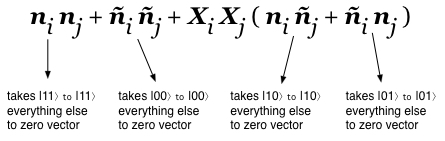
\includegraphics[width=0.5\textwidth]{FIGURES/Mermin_(2007)_Support_(Eq_135).jpg}
  \caption{Summary interpretation of terms in Mermin's (2007) Eq (1.35), pg 12. For the $i$th and $j$th Cbits each being $|1\rangle$, all the terms but the first collapse to zero vectors and that first term returns the original input. For the $i$th and $j$th Cbits each being $|0\rangle$, all the terms but the second one collapse to zero vectors and the second term returns the original input. The third and fourth terms serve as identity multipliers for inputs $|10\rangle$ and $|01\rangle$ respectively, then the $X_iX_j$ operators ``flip'' the individual states to produce $|01\rangle$ and $|10\rangle$ respectively. The overall effect, then is to take the targeted $i,j$ pair of Cbits and swap their values.}
  \label{fig:Eq135Interpret}
\end{figure}

%%%%%%%%%%%%%%%%%%%
%   1.40          %
%%%%%%%%%%%%%%%%%%%

\vspace{0.25in}

\textbf{EQ 1.40 (The cNOT operator in terms of $\bm{X}$ and $\bm{Z}$)}\par

\vspace{0.25in}

Using the $\bm{X}$ (NOT or ``flip'') and $\bm{Z}$ operators:

\begin{align*}
  \bm{X} &= \begin{pmatrix}0 & 1\\1 & 0\end{pmatrix}\\
  \bm{Z} &= \bm{\widetilde{n}} - \bm{n} = \begin{pmatrix}1 & 0\\0 & -1\end{pmatrix}
\end{align*}

Mermin notes that the cNOT operator can be expressed as:

\begin{align*}\tag{1.40}
    \bm{C}_{ij}
    &= \frac{1}{2}(\bm{1} + \bm{Z}_i)
       + \frac{1}{2}\bm{X}_j(\bm{1} - \bm{Z}_i)\\
    &= \frac{1}{2}(\bm{1} + \bm{X}_j)
       + \frac{1}{2}\bm{Z}_i(\bm{1} - \bm{X}_j)
\end{align*}

where ``The second form follows from the first because $\bm{X}_j$ and $\bm{Z}_i$ commute when $i \ne j$'' [pg. 13]

\vspace{0.125in}

To see this more clearly, we expand the first line, rearrange, and then use the commutativity of $\bm{X}_j$ and $\bm{Z}_i$ as follows:

\begin{align*}
    \bm{C}_{ij}
    = \frac{1}{2}(\bm{1} + \bm{Z}_i)
       + \frac{1}{2}\bm{X}_j(\bm{1} - \bm{Z}_i)
    & = \frac{1}{2}\bm{1} + \frac{1}{2}\bm{Z}_i
        + \frac{1}{2}\bm{X}_j\bm{1} - \frac{1}{2}\bm{X}_j\bm{Z}_i
        \text{ [expanding]}\\
    & = \frac{1}{2}\bm{1} + \frac{1}{2}\bm{X}_j\bm{1}
         + \frac{1}{2}\bm{Z}_i - \frac{1}{2}\bm{X}_j\bm{Z}_i
        \text{ [rearranging]}\\
    & = \frac{1}{2}\bm{1} + \frac{1}{2}\bm{X}_j\bm{1}
         + \frac{1}{2}\bm{Z}_i - \frac{1}{2}\bm{Z}_i\bm{X}_j
        \text{ [commuting }\bm{X}_j\text{ and }\bm{Z}_i\text{]}\\
    &= \frac{1}{2}(\bm{1} + \bm{X}_j)
       + \frac{1}{2}\bm{Z}_i(\bm{1} - \bm{X}_j)
       \text{ [factoring]}
\end{align*}

\vspace{0.125in}

%%%%%%%%%%%%%%%%%%%
%   1.41          %
%%%%%%%%%%%%%%%%%%%

\vspace{0.25in}

\textbf{EQ 1.41 (The Marsh-Hadamard Transformation $\bm{H}$)}\par

\vspace{0.25in}

The Hadamard (or Marsh-Hadamard) transformation $\bm{H}$ is defined by:

\[\tag{1.41}
\bm{H} = \frac{1}{\sqrt{2}}(\bm{X} + \bm{Z}) = \frac{1}{\sqrt{2}}\begin{pmatrix} 1 & 1 \\ 1 & -1 \end{pmatrix}
\]

Mermin observes that (pg 14), since $\bm{X}^2 = \bm{Z}^2 = \bm{1}$ and $\bm{X}\bm{Z} = -\bm{Z}\bm{X}$, one easily shows from the definition (1.41) of $\bm{H}$ in terms of $\bm{X}$ and $\bm{Z}$ that
\[\tag{1.42}
\bm{H}^2 = \bm{1}
\]
and that
\[\tag{1.43}
\bm{H}\bm{X}\bm{H} = \bm{Z},\quad\bm{H}\bm{Z}\bm{H} = \bm{X}.
\]
So let's do the math and show these things. From (1.41) and the anti-commutativity of $\bm{X}$ and $\bm{Z}$ we have:
\begin{align*}
    \bm{H}^2
    &= \frac{1}{2}(\bm{X} + \bm{Z})^2\\
    &= \frac{1}{2}(\bm{X}^2 + \bm{X}\bm{Z} + \bm{Z}\bm{X} +  \bm{Z}^2)\\
    &= \frac{1}{2}(\bm{X}^2 + \bm{X}\bm{Z} - \bm{X}\bm{Z} +  \bm{Z}^2)\\
    &= \frac{1}{2}(\bm{X}^2 + \bm{Z}^2)\\
    &= \frac{1}{2}(\bm{1} + \bm{1})\\
    &= \bm{1}
\end{align*}
We also have:
\begin{align*}
    \bm{H}\bm{X}\bm{H}
    &= \frac{1}{\sqrt{2}}(\bm{X} + \bm{Z})\bm{X}(\frac{1}{\sqrt{2}})(\bm{X} + \bm{Z})\\
    &= \frac{1}{2}(\bm{X} + \bm{Z})\bm{X}(\bm{X} + \bm{Z})\\
    &= \frac{1}{2}(\bm{X}^2 + \bm{Z}\bm{X})(\bm{X} + \bm{Z})\\
    &= \frac{1}{2}(\bm{X}^2\bm{X} + \bm{X}^2\bm{Z} + \bm{Z}\bm{X}^2 + \bm{Z}\bm{X}\bm{Z})\\
    &= \frac{1}{2}(\bm{X}^2\bm{X} + \bm{X}^2\bm{Z} + \bm{Z}\bm{X}^2 - \bm{Z}^2\bm{X})\\
    &= \frac{1}{2}(\bm{X} + \bm{Z} + \bm{Z} - \bm{X})\\
    &= \bm{Z}
\end{align*}
and
\begin{align*}
    \bm{H}\bm{Z}\bm{H}
    &= \frac{1}{\sqrt{2}}(\bm{X} + \bm{Z})\bm{Z}(\frac{1}{\sqrt{2}})(\bm{X} + \bm{Z})\\
    &= \frac{1}{2}(\bm{X} + \bm{Z})\bm{Z}(\bm{X} + \bm{Z})\\
    &= \frac{1}{2}(\bm{X}\bm{Z} + \bm{Z}^2)(\bm{X} + \bm{Z})\\
    &= \frac{1}{2}(\bm{X}\bm{Z}\bm{X} + \bm{X}\bm{Z}^2 + \bm{Z}^2\bm{X} + \bm{Z}^2\bm{Z})\\
    &= \frac{1}{2}(-\bm{X}^2\bm{Z} + \bm{X}\bm{Z}^2 + \bm{Z}^2\bm{X} + \bm{Z}^2\bm{Z})\\
    &= \frac{1}{2}(-\bm{Z} + \bm{X} + \bm{X} + \bm{Z})\\
    &= \bm{X}
\end{align*}

\vspace{0.125in}

%%%%%%%%%%%%%%%%%%%
%   1.44          %
%%%%%%%%%%%%%%%%%%%

\vspace{0.25in}

\textbf{EQ 1.44 (Transforming $\bm{C}_{ij}$ to $\bm{C}_{ji}$ using the Marsh-Hadamard Transformation $\bm{H}$)}\par

\vspace{0.25in}

Mermin writes (pg 14) that ``it follows from (1.43), together with (1.40) and (1.42), that''

\[\tag{1.44}
\bm{C}_{ji} = (\bm{H}_i\bm{H}_j)\bm{C}_{ij}(\bm{H}_i\bm{H}_j)
\]

Recall from (1.40) that $\bm{C}_{ij} = \frac{1}{2}[(\bm{1} + \bm{Z}_i) + \bm{X}_j(\bm{1} - \bm{Z}_i)]$ and thus $\bm{C}_{ji} = \frac{1}{2}[(\bm{1} + \bm{Z}_j) + \bm{X}_i(\bm{1} - \bm{Z}_j)]$. So we can gradually process the RHS of (1.44), keeping in mind the commutativity of the matrix multiplications when the subscripts do not match:

\begin{align*}
(\bm{H}_i\bm{H}_j)\bm{C}_{ij}(\bm{H}_i\bm{H}_j)
&= \frac{1}{2}(\bm{H}_i\bm{H}_j)[(\bm{1} + \bm{Z}_i) + \bm{X}_j(\bm{1} - \bm{Z}_i)](\bm{H}_i\bm{H}_j)\\
&= \frac{1}{2}[\bm{H}_i\bm{H}_j + \bm{H}_i\bm{H}_j\bm{Z}_i + \bm{H}_i\bm{H}_j\bm{X}_j - \bm{H}_i\bm{H}_j\bm{X}_j\bm{Z}_i](\bm{H}_i\bm{H}_j)\\
&= \frac{1}{2}[\bm{H}_i\bm{H}_j\bm{H}_i\bm{H}_j + \bm{H}_i\bm{H}_j\bm{Z}_i\bm{H}_i\bm{H}_j + \bm{H}_i\bm{H}_j\bm{X}_j\bm{H}_i\bm{H}_j - \bm{H}_i\bm{H}_j\bm{X}_j\bm{Z}_i\bm{H}_i\bm{H}_j]\\
&=\tag{commuting} \frac{1}{2}[\bm{H}_i\bm{H}_i\bm{H}_j\bm{H}_j
+ \bm{H}_j\bm{H}_i\bm{Z}_i\bm{H}_i\bm{H}_j
+ \bm{H}_i\bm{H}_j\bm{X}_j\bm{H}_j\bm{H}_i
- \bm{H}_j\bm{X}_j\bm{H}_i\bm{Z}_i\bm{H}_i\bm{H}_j]\\
&=\tag{simplifying using (1.42) and (1.43)} \frac{1}{2}[(\bm{1})(\bm{1})
+ \bm{H}_j\bm{X}_i\bm{H}_j
+ \bm{H}_i\bm{Z}_j\bm{H}_i
- \bm{H}_j\bm{X}_j\bm{X}_i\bm{H}_j]\\
&=\tag{commuting} \frac{1}{2}[\bm{1}
+ \bm{H}_j\bm{H}_j\bm{X}_i
+ \bm{H}_i\bm{H}_i\bm{Z}_j
- \bm{H}_j\bm{X}_j\bm{H}_j\bm{X}_i]\\
&=\tag{simplifying using (1.42) and (1.43)} \frac{1}{2}[\bm{1}
+ \bm{X}_i
+ \bm{Z}_j
- \bm{Z}_j\bm{X}_i]\\
&=\tag{commuting} \frac{1}{2}[\bm{1}
+ \bm{Z}_j
+ \bm{X}_i
- \bm{X}_i\bm{Z}_j]\\
&=\tag{factoring} \frac{1}{2}[(\bm{1} + \bm{Z}_j)
+ \bm{X}_i (\bm{1} - \bm{Z}_j)]\\
&= \bm{C}_{ji}
\end{align*}


% ===================== %
%   (2^n)! Typo pg 19   %
% ===================== %

\vspace{0.25in}

\textbf{\large $(2^n)!$ and Text Typo on pg 19}\par

\vspace{0.25in}

There appears to be a typo or mis-statement in the paragraph just before Eq (1.68) on pg 19. Mermin writes that ``The most general reversible $n$-Cbit oepration in a classical computer is a permutation of the $(2^n)!$ different classical-basis states,'' but there should be just $2^n$ basis states and $(2^n)!$ \textit{permutations} (that seems clear from the next sentence and from the earlier discussion of permutations on pg 9 (beginning in the paragraph just before Eq. (1.19)).

% ============================ %
%  The Generalized Born Rule   %
%  Eq. 1.76                    %
% ============================ %

\vspace{0.25in}

\textbf{\large \S1.9 The Generalized Born Rule, Eq. (1.76)}\par

\vspace{0.25in}

The presentation and equation for the generalized Born rule is difficult to follow at first, and thus worthy  of some careful elaboration and examples. As Mermin remarks (pg 28), this stronger form of the Born rule ``applies when one measures only a single one of $n+1$ Qbits, by sending it through a standard 1-Qbit measurement gate.''

Mermin begins by noting that any state $|\Psi\rangle_{n+1}$ of all $n+1$ Qbits can be represented in the form:

\[\tag{1.76}
|\Psi\rangle_{n+1} =
  \alpha_0 |0\rangle |\Phi_0\rangle_n
  + \alpha_1 |1\rangle |\Phi_1\rangle_n,
  \hspace{0.25in}|\alpha_0|^2 + |\alpha_1|^2 = 1
\]

where $|\Phi_0\rangle_n$ and $|\Phi_1\rangle_n$ are normalized but not necessarily orthogonal.

\vspace{0.125in}

As we shall see, this is a way to re-express the $(n+1)$-Qbit system state $|\Psi\rangle_{n+1}$ in terms of the left-most Qbit plus the collection of the remaining $n$ Qbits.

\vspace{0.125in}

Note that the $|0\rangle$ and $|1\rangle$ in (1.76) are actually the Cbit (or equivalent Qbit) states $|0\rangle_1$ and $|1\rangle_1$, respectively, which will then give the correct sizes for the result of the tensor products implied on the right-hand side of (1.76). To be more explicit: $|\Psi\rangle_{n+1}$ (\textit{i.e.}, the left-hand side of (1.76)) can be represented as a $2^{n+1}\times 1$ column vector. From the right-hand side, $|0\rangle$ is a $2\times 1$ column vector and $|\Phi_0\rangle_{n}$ is a $2^n \times 1$ column vector. The tensor product $|0\rangle |\Phi_0\rangle_{n}$ is thus a $2(2^n)\times 1 = 2^{n+1}\times 1$ column vector. Similarly, $|1\rangle |\Phi_1\rangle_{n}$ is also a $2^{n+1}\times 1$ column vector.

\vspace{0.125in}

Letting:

\[\tag{1.77}
  |\Psi\rangle_{n+1} = \sum_{x=0}^{2^{n+1}-1}\gamma(x)|x\rangle_{n+1},
  \text{ where }
  \sum_{x=0}^{2^{n+1}-1}|\gamma(x)|^2 = 1,
\]

the states $|\Phi_0\rangle_n$ and $|\Phi_1\rangle_n$ are given by

\[\tag{1.78}
  |\Phi_0\rangle_n = \frac{1}{\alpha_0}
  \sum_{x=0}^{2^{n}-1}\gamma(x)|x\rangle_{n}
  \text{ and }
  |\Phi_1\rangle_n = \frac{1}{\alpha_1}
  \sum_{x=0}^{2^{n}-1}\gamma(2^n + x)|x\rangle_{n},
\]

where

\[\tag{1.79}
\alpha^2_0 = \sum_{x=0}^{2^{n}-1}|\gamma(x)|^2
\text{ and }
\alpha^2_1 = \sum_{x=0}^{2^{n}-1}|\gamma(2^n + x)|^2.
\]

The first term on the right-hand side of (1.76), then, gives:

\[
  \alpha_0 |0\rangle |\Phi_0\rangle_n
  =
  \alpha_0 \begin{pmatrix}1\\0\end{pmatrix}
  \otimes
  \begin{pmatrix}\gamma(0)/\alpha_0\\
                 \gamma(1)/\alpha_0\\
                 \gamma(2)/\alpha_0\\ \vdots \\
                 \gamma(2^n - 1)/\alpha_0\end{pmatrix}
  =
  \begin{pmatrix}\gamma(0)\\
                 \gamma(1)\\
                 \gamma(2)\\ \vdots \\
                 \gamma(2^n - 1) \\
                 0 \\ 0 \\ \vdots \\ 0
                 \end{pmatrix}
\]

giving a $2^{n+1}\times 1$ column vector, the last half of which consists of all zero entries. The second term on the right-hand side of (1.76) gives:

\[
  \alpha_1 |1\rangle |\Phi_1\rangle_n
  =
  \alpha_1 \begin{pmatrix}0\\1\end{pmatrix}
  \otimes
  \begin{pmatrix}\gamma(2^n)/\alpha_1\\
                 \gamma(2^n + 1)/\alpha_1\\
                 \gamma(2^n + 2)/\alpha_1\\ \vdots \\
                 \gamma(2^n + 2^n - 1)/\alpha_1\end{pmatrix}
  =
  \begin{pmatrix}0 \\ 0 \\ \vdots \\ 0 \\
                 \gamma(2^n)\\
                 \gamma(2^n + 1)\\
                 \gamma(2^n +2)\\ \vdots \\
                 \gamma(2^{n + 1} - 1)
                 \end{pmatrix}
\]

giving a $2^{n+1}\times 1$ column vector, the first half of which consists of all zero entries.

\vspace{0.25in}

\textbf{\large Some Notation}\par

$\psi$ (psi) versus $\phi$ (phi) versus $\varphi$ (phi variant style)


% =============== %
%  Bibliography   %
% =============== %

\printbibliography

\end{document}